\documentclass[a4paper,12pt]{article}
\usepackage{t1enc}
\usepackage[longnamesfirst, round]{natbib}  % Bindet den natbib-standard fuer das Zitieren ein
\usepackage{epsfig}
\usepackage[latin1]{inputenc}   % Ermoeglicht Sonderzeichen direkt einzugeben
\usepackage[T1]{fontenc}        % Garantiert saubere Worttrennung bei Umlauten etc.
\usepackage{color}              % Farbpaket
\usepackage{amsmath,amsfonts,amssymb}   % ermoeglicht mathematische Sonderzeichen
\usepackage{ngerman}           % neue deutsche Rechtschreibung
\usepackage[english]{babel}     %
\usepackage{ae}                 %
\usepackage{graphicx}           % Ermoeglicht das Einbinden von Bildern in allen Formaten
\usepackage{longtable}          % zum erstellen von Tabellen ber mehrere Seiten
\usepackage{multirow}           % zum Verbinden von Zeilen innerhalb einer Tabelle
%\usepackage{pictexwd}           % PicTex, ein Graphikpaket
%\usepackage{pst-all, multido}   % psTricks, ein Graphikpaket
\usepackage{url}



% ________________ EINRICHTEN DES DOKUMENTS ______________________%

\bibliographystyle{plainnat}    % legt den Stil fuer das Inhaltsverzeichnis fest

\oddsidemargin 0.1in \evensidemargin 0.1in \textwidth 15.5cm \topmargin -0.4in \textheight 24.5cm
\parindent 0cm      % legt die Seitenraender fest

\pagestyle{plain}          % leere Kopfzeile, Seitennummer in der Mitte der Fusszeile

\newcommand{\bs}{\boldsymbol}  % shortcut zur Erzeugung von fetten Sympolen in der Mathe-Umgebung

\renewcommand{\baselinestretch}{1.25}
% 1,5 -facher Zeilenabstand (Standard ist 1,2-facher Zeilenabstand, also 1,2*1,25 = 1,5



\begin{document}

% ________________ TITELSEITE ______________________%


\pagenumbering{roman}   % roemische Zahlen zur Seitennumerierung

\begin{titlepage}       % Umgebung fuer Titelseite, frei gestaltbar

\thispagestyle{empty}   % keine Numerierung auf Titelseite


\begin{center}
\vspace*{2.5cm}
{\bf  \Large The Distribution of Wealth \\in a Life-Cycle Model with Durables} \\
\vspace*{3cm} 
Master Thesis \\ in Economics \\
Prof. Dr. Thomas Hintermaier  \\
\vspace*{0.5cm} 
Summer Term 2017\\
\end{center}

\vfill
\begin{flushright}
   \emph{Eric Lustenberger} \\
    \emph{Heckenweg 38}\\
    \emph{3007 Bern}\\
   \emph{Student Number}\\
 \emph{Economics}\\

\end{flushright}



% 
% \begin{center}
% $ $			% oeffnet und schliesst eine Matheumgebung (Trick, um den Titel nach unten zu rutschen
% \vspace{4cm}
% 
% {\LARGE TITEL}
% \vskip 4cm
% 
% Diese Seite ist frei gestaltbar
% \end{center}

\end{titlepage}

\newpage                % erzwingt an dieser Stelle einen Seitenumbruch



% ________________ INHALTSVERZEICHNIS ______________________%


% \tableofcontents   %fuegt Automatisch ein Inhaltsverzeichnis ein
% 
% \newpage
% 


% ________________ HAUPTTEIL ______________________%


\pagenumbering{arabic}      % Seitenzahlen wieder arabisch numerieren
\setcounter{page}{1}        % Ruecksetzen des Seitenzahlzaehlers auf 1


\section{\"Introduction}
\label{Chapter1}

\subsection{Unter\"Uberschrift}

\subsubsection*{UnterUnter\"Uberschrift}



Hier steht mal ein Text. Eine M\"oglichkeit des Zitierens ist, direkt
im Text die Quelle anzugeben \citep[see][pp.225-369]{key1}.
Andererseits schreiben \cite{key2}, dass man auch so zitieren kann.

In der Matheumgebung kann der oben (im Latex-Quellcode) genannte Shortcut verwendet
werden, um aus einem normalen $\beta$ ein fettes $\bs \beta$ zu
machen. Wichtige Gleichungen, die nochmal verwendet werden, sollten nummeriert werden, z.B.
\begin{equation}
\label{eq:ols}
   b = (x'x)x'y \;.
\end{equation}

Nebens\"achlicheres, auf das man sich nicht mehr bezieht, bleibt unnummeriert, also 
\begin{equation*}
   a = 1\;.
\end{equation*}
Nun kann man direkt auf die erste Gleichung als Gleichung~\eqref{eq:ols} verweisen mittels des zugewiesenen labels. In gleicher Weise kann man auf die Graphik~\ref{fig:ersteGraphik} bzw. Graphik~\ref{fig:andereGraphik} verweisen. Die Tilde zwischen \glqq Graphik\grqq{} und \glqq \verb|\ref{fig:andereGraphik}|\grqq{} verhindert, dass bei Zeilenumbr\"uchen die Zahl als erstes alleine in die neue Zeile rutscht. Ganz analog f\"ur die Tabelle~\ref{tab:Tabelle}. 



\section{Ben\"otigte Programme}

unter Windows:
\begin{itemize}
   \item Miktex (\url{http://miktex.org/})
   \item ein Editor, je nach Geschmack z.B. WinEdt (\url{http://www.winedt.com/}; kostenpflichtige Studentenversion) oder einen der vielen anderen verf\"ugbaren, z.B. TeXnicCenter (\url{www.texniccenter.org/})
   \item ghostview und ghostscript (\url{http://pages.cs.wisc.edu/~ghost/}
\end{itemize}
unter Linux:
\begin{itemize}
   \item Latex ist in den meisten Verteilungen enthalten, z.B. tetex in Suse (ggf. \"uber yast nachinstallieren)
   \item als Editor empfiehlt sich z.B. Kile
\end{itemize}
f\"ur die Literatur:\\
z.B. JabRef (\url{http://jabref.sourceforge.net/})


\section{Pr\"asentationen}

Beispiele f\"ur Pr\"asentationen mit dem Beamer-Style:

\url{http://www.informatik.uni-freiburg.de/~frank/latex-kurs/latex-kurs-3/Latex-Kurs-3.html}


\section{Literature Overview}
\label{Chapter2}

Investigate empirical predictions of the life-cycle incomplete markets model (\cite{Gourinchas&Parker2002}; \cite{cagetti2003}; \cite{castaneda2003}; \cite{yang2009}; \cite{kaplan2010}; \cite{hintermaier2011}), thus contribute to the literature that (note copy paste.... demonstrate that a plausibly parameterized version of their models can quantitatively explain empirical findings as arising from rational choices of consumers facing an increasing wage profile and income uncertainty.)
The model is based on the classic income-fluctuation problem in which the consumer faces a stochastic income process and decides in every period how much to save and how much to consume. Important contributions to the literature are Deaton (1991), Carroll (1992,1997), \cite{Gourinchas&Parker2002}. (note copy paste... Following Bewley (1986), this problem has been embedded by Huggett (1993) and Aiyagari (1994) into a general equilibrium framework, giving rise to the endogenous determination of the interest rate as well as a nontrivial income, wealth, and consumption distribution at equilibrium.)
(Note copy paste... Furthermore, this paper relates to other literature such as: 
Endogenous borrowing constraint: The specification of the borrowing constraint  in \cite{FV&K2011} is adapted from the recent endogenous incomplete-markets literature: Kehoe and Levine (1993), Kocherlakota (1996), Krueger and Perri (1999, 2006), and Alvarez and Jermann (2000). Lustig (2004) also has a model with durable assets and an endogenous borrowing constraint to explain the equity premium puzzle, however agents have full access to Arrow securities and are infinitely lived.
Literature on optimal portfolio choice in the presence of consumer durables: Grossman and Laroque (1990), Eberly (1994), Chah et al. (1995), and Flavin and Yamashita (2002).)

Note: missing citations, not all of the above are cited properly!!!!!

Literature on wealth distribution!!!!! 

\section{The Life-Cycle Model}
\label{Chapter3}
In the following section I discuss the economic model considered and outline the most important considerations made within the literature. Firstly, I discuss the life-cycle modeling and the literature, which applies life-cycle and to be more exact imperfect markets models in the context of wealth distributions. Secondly, I present my modeling choices and solution methods applied for this particular problem. 
\subsection{Modeling Literature}

\subsection{The Model}
Before going into a more detailed description of the model at hand it is important to understand the modelling choice. Why a life-cycle model with an imperfect market structure? Why include durables as an  additional asset choice to the more standard approach, which does summarize all assets in a one period bond, such as for example \cite{hintermaier2011}? 

To answer the first question I will mainly refer to the the literature. The second will be discussed in a more detailed manner in the following section, which treads the life-cycle profiles and especially the importance of modeling durables. 

\subsubsection{Imperfect market structure}
The choice of an exogenously determined imperfect market structure allows for a straight forward answer. It comes down to the economic question one poses. The aim here is to demonstrate that such a model can quantitatively explain the empirical net-wealth distribution in the US. The role the imperfect market structure, entering as a limited choice of assets to fully insure against idiosyncratic wage shocks, poses, is thus to produce an endogenous wealth distribution. The savings are fist and foremost driven by a precautionary motive to insure for future wage shocks. Knowing that the income may drop in the future consumers save today to achieve a more stable consumption across their live. In a complete market framework consumers could perfectly diversify away idiosyncratic risks \citep{a&w2010}  (and thus would not build a buffer stock of savings for future shocks.) (???????? is this exact?????)
The hypothesis of the complete market framework has been rejected by the vast majority of empirical research \citep{a&w2010}. \cite{deaton1994} show that the life cycle profile of consumption inequality is increasing with age, a fact that would be inconsistent with complete markets. While in some rare cases - such as when only studying aggregates, it may still be sufficient to consider a complete market framework, when considering wealth-distributive questions, the imperfect market assumption is both necessary from a theoretical perspective and well-founded from an empirical perspective. It remains to discuss the whether it makes sens to treat distributive issues from a life-cycle point of view.

\subsubsection{Life-Cycle}

As \cite{deaton1994} show, consumption inequality seems to vary with age. Further empirical research does support these findings, indicating that some of the differences in earnings, income, and wealth across households can be attributed to differences in the household's age \cite{rios2016} (FIND BETTER REFERENCES?). \cite{hintermaier2011} Show that the average net-wealth increases with wealth and that the dispersion of wealth falls with age. 
Moreover, there is a vast theoretical literature using a different versions of the life-cycle model to discuss distributive questions.  \cite{Gourinchas&Parker2002}; \cite{cagetti2003}; \cite{castaneda2003}; \cite{yang2009}; \cite{kaplan2010};\cite{hintermaier2011} (CITE MORE RECENT LITERATURE!!!)
while there are also some that use infinite horizon models....

Finally, the choice to study the empirical validity of a life-cycle model, which produces a net-wealth distribution arising from rational choices of consumers subject to income uncertainty, moreover allows for a detailed analysis of consumption and savings behavior over a person's live-cycle. A coherent framework incorporating the behavior of household's over their lifespan is paramount for the study of re-distributive policies. (Cite....)
These factors thus support the choice of a life-cycle model. 


\subsubsection{Partial Equilibrium}
Last but not least, partial equilibrium as modeling choice has to be discussed briefly. (????????????????)



\subsubsection{Consumer's Problem}
As established above, the model in question is a life-cycle model with an imperfect market structure. I closely follow \cite{hintermaier2011} adding consumption durables to the model. In order to facilitate comparability, I will closely follow the notation used in their paper.

(Copy paste: In this model there is a continuum of risk-averse consumers who have a finite time horizon. These consumers make consumption and savings decisions between age 26 and age 90 when they die with certainty. Befor age 90, the probability of death at age j is $\delta_{j} < 1$. \\ 
Consumers retire with certainty after age 65 is completed. We let $T^{r}$ denote the first period of retirement. Before retirement, labor income $y_{ij}$ is stochastic as described by Eqs. (1) and (2). After retirement, consumers receive individual-specific retirement benefits $b_{i}$. We discuss in detail in the next section how these retirement benefits are determined.  \\
Consumers derive utility from a non-durable good $c$. The utility function is denoted by $u(c)$ and is assumed to be strictly concave and increasing. Consumers have access to a risk-free asset $a$ which earns interest $r$ so that markets are incomplete given that labor income is stochastic before retirement. As consumers cannot fully diversify their risk, different histories of labor income shocks imply different net worth positions. Moreover, the consumption and savings decision depends on the age of consumers which determines the position in the life cycle. The model is thus well suited to match the empirical facts about net worth mentioned in the previous section since it produces an endogenous net worth distribution for consumers with different histories of income shocks and different age. 

\paragraph{The recursive formulation of the household problem}


\subsubsection{Numerical algorithm}


\subsubsection{Comparing the simulation output with SCF data}

\subsubsection{Calibration}







\section{Life-Cycle Profiles}
\label{Chapter4}
\section{The Wealth Distribution}
\label{Chapter5}
\section{Conclusion}
\label{Chapter6}
%_________________ ENDE DES HAUPTTEILS_________________%


\newpage


%_________________ Literaturverzeichnis _______________%

\addcontentsline{toc}{section}{References}        % Fuegt im Inhaltsverzeichnis "References" hinzu
\bibliography{bib_thesis}                         % Erstellt Literaturverzeichnis (bindet das file bib_thesis.bib ein

%_________________ Platz fuer Graphiken und Tabellen _______________%

\newpage

% Einfuegen einer Grafik
\begin{figure}
\caption{titel der Graphik} 
\label{fig:ersteGraphik}	%label, um spaeter auf die Graphiknummer zugreifen zu koennen
\centering
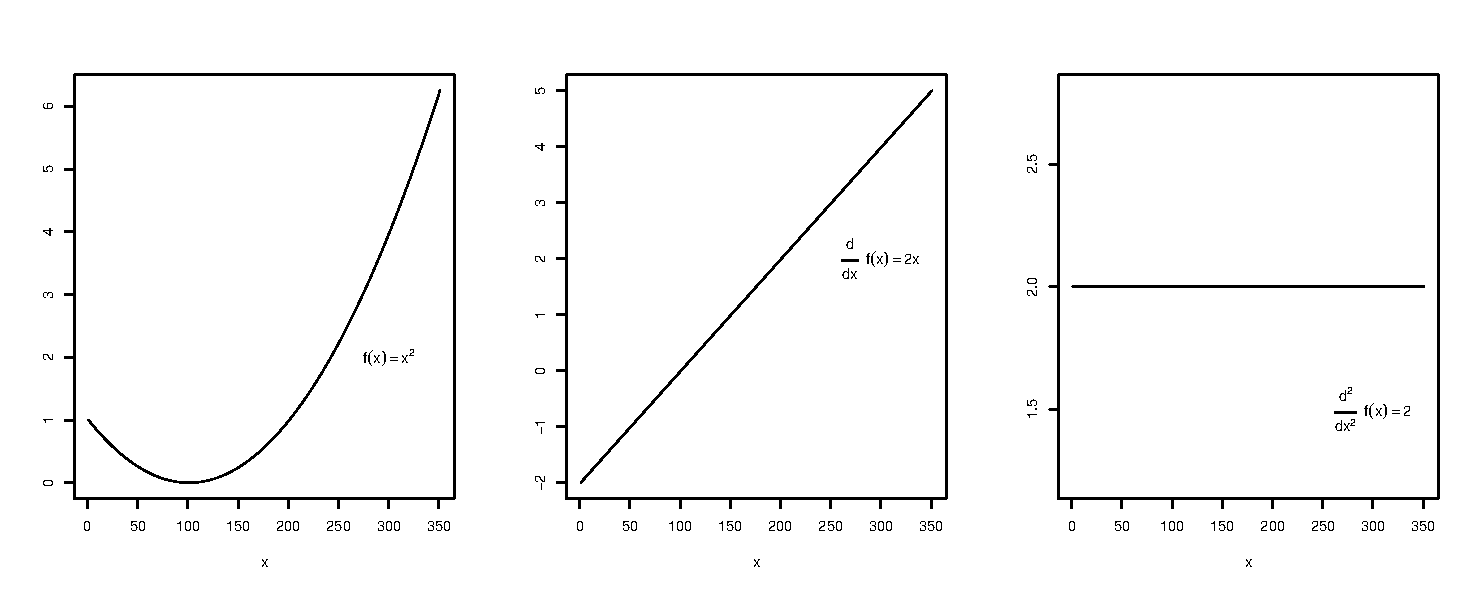
\includegraphics[width=6.5cm]{abb1.png}  % width legt Breite der Graphik fest

\begin{minipage}{0.8\linewidth}
\footnotesize{die Graphik sollte beschrieben werden, sodass man ohne den Text vorne zu lesen wei\ss{}, worum es geht: panel 1 zeigt die Funktion, panel 2 die erste Ableitung und Panel 3 die zweite Ableitung}
\end{minipage}

\end{figure}

\begin{figure}
\caption{titel der Graphik}
\label{fig:andereGraphik} \centering
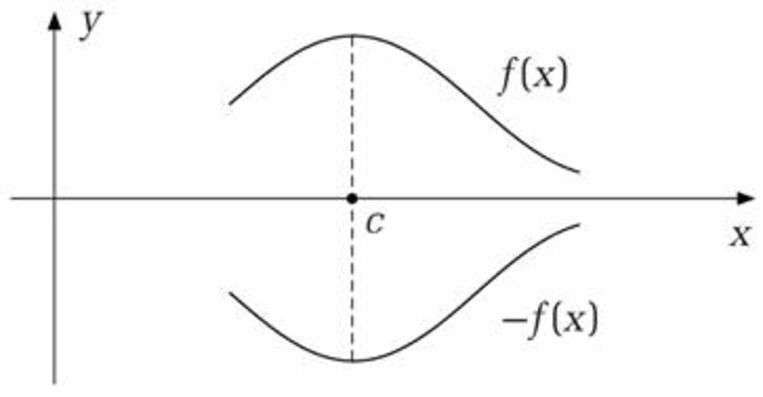
\includegraphics[angle=90,height=6.5cm]{abb2.jpg}  % angle dreht die Graphik, falls noetig; height legt die Hoehe der Graphik fest

\end{figure}

\begin{table}
\caption{Der Title der Tabelle}
\label{tab:Tabelle}
\centering
 \begin{tabular}{lc|r}
   Eine & kleine & Tabelle\\
\hline
   Text links & mittig & oder rechts \\
   & unterstrichen  & \\
\cline{2-2}
   \multicolumn{2}{c|}{\"uber zwei Spalten} & dritte Spalte \\
\end{tabular}   
\end{table}

   





\end{document}
